\chapter{研发迭代过程}

\section{测试记录}
% 官方要求：对机器人各项功能点进行测试验收，记录测试环境、测试设备等信息。
\subsection{功能一：重复度测试}
\subsubsection{测试内容}
针对枪管定心各方案的重复度效果进行实际对比，验证关键参数的改动是否会对实际重复度的效果产生符合设想的影响。

\subsubsection{测试环境与设备}
\paragraph{测试环境}
环境选择的标准是：
\begin{itemize}
    \item 尽量选择室内环境，室外环境不适合弹丸的收集且通常卫生条件不够好，导致弹丸每次使用后表面会附着大量杂物从而影响后续的使用，并且室内环境可以避免自然风对弹道的影响。
    \item 尽量选择干燥环境，同样是出于避免弹丸表面附着大量杂物的考虑，同时避免机器人在潮湿环境下出现问题。
    \item 由于实验楼可供选择的测试地点不多，在找到合适的场地时，必须注意周边的实验室是否有研究生或者老师正在办公/休息，提前打好招呼，避免引起不满导致不必要的麻烦。
    \item 尽量选择光照条件较好的环境，极大地方便测试的同时，确保晚上也不会因为光照条件差导致整体测试效率降低。
\end{itemize}
布置环境时应注意的事项：
\begin{itemize}
    \item 重复度效果体现在A4纸上，由于在软质表面上，A4纸和复写纸在$\qty{47}{\mm}$弹丸以$\qty{30}{\metre\per\second}$的速度击打时容易破损，通常会采用“硬质表面-A4纸（记录用）-复写纸-多张A4纸（保护用）”的形式。
    \item 若使用发射测试架验证重复度效果，发射测试架本身与A4纸（记录用）的相对位置必须保证没有变化，可以通过重物压制等方式达到效果。
    \item 若使用机器人整体去验证重复度效果，则需要用机械固定的方式稳定机器人Pitch轴与Yaw轴，如\figref{fig:Pitch轴固定展示}所示，完全排除控制因素对于机械重复度效果的影响。    
\end{itemize}

\begin{figure}[hbt!]
    \centering 
    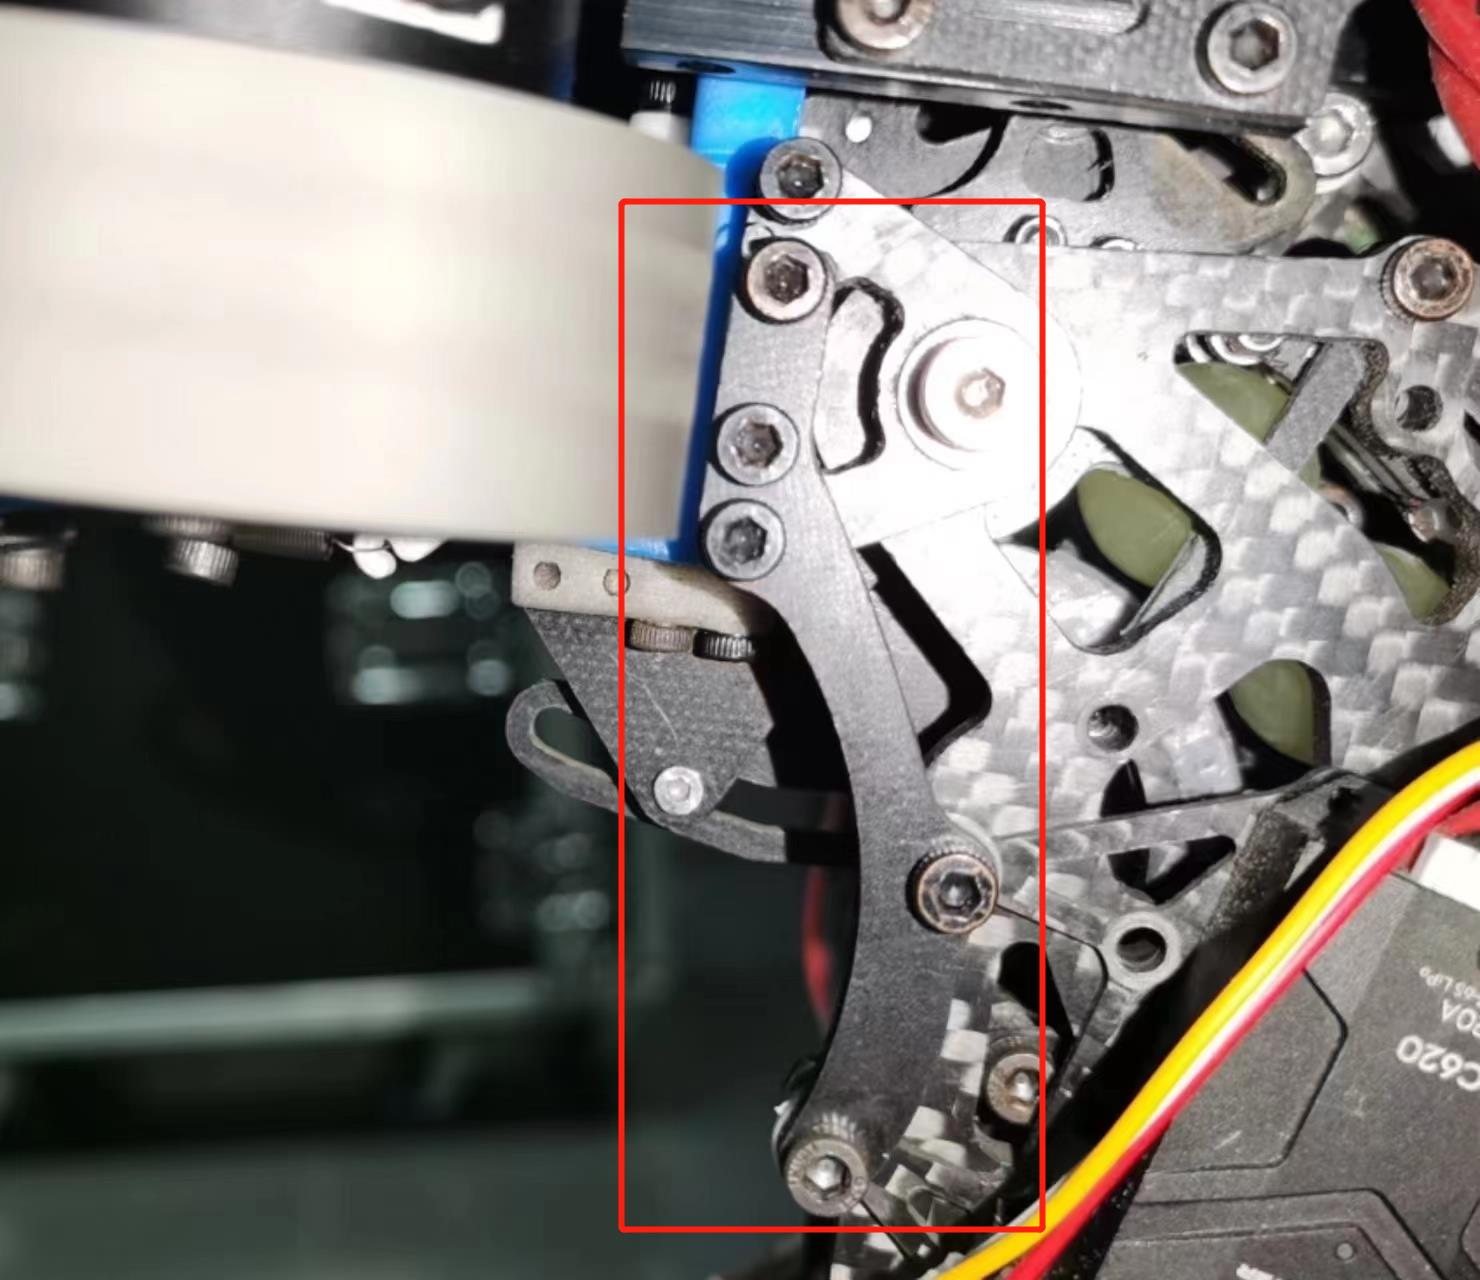
\includegraphics[width=0.5\columnwidth]{figure/研发迭代过程/Pitch轴固定展示.jpg}
    \caption{Pitch轴固定展示}
    \label{fig:Pitch轴固定展示}
\end{figure} 

\paragraph{注意事项}


当双发情况严重，且目前机构为已验证过可用的稳定机构，则自行排除以下方面的错误：
\begin{itemize}
    \item offset（拨盘位置初始偏移量）数值是否被调整。
    \item 拨盘减速比是否正确。
    \item 单发限位模块运作是否正常。
    \item 拨弹空转时运作是否正常。
    \item 拨盘是否超调。
\end{itemize}

当卡弹情况严重，且目前机构为已验证过的可用稳定机构，则自行排除以下方面的错误：
\begin{itemize}
    \item 断控，手动转动拨盘，若无法拨动则确定为机械问题。
    \item 弹链是否出现异物。
    \item 中心供弹机构是否出现异物。
    \item 拨弹空转时运作是否正常。
    \item 单发限位模块运作是否正常。
\end{itemize}

\paragraph{设备}

\begin{longtable}[htbp!]{ m{4cm}<{\centering}  m{9cm}<{\centering} }
\hline
设备名称  &   设备用途       \\
\hline
\endfirsthead
\hline
设备名称  &   设备用途       \\
\hline
\endhead
\hline
\multicolumn{2}{r}{接下页}
\endfoot
\caption{设备}
\label{tab:设备}
\endlastfoot
%   填这里
 \hline
 A4纸 & 用于记录弹丸击打的具体范围，直观地展示其散布\\
 \hline 
 发射测试架 & 用于上供弹步兵弹丸定心机构的验证，同时验证供弹方式不同对于统一弹丸定心机构的不同影响 \\
 \hline
 复写纸 & 用于辅助记录弹丸击打的具体范围，直观地展示其散布\\
 \hline
 金银矿石 & 用于将机器人垫高，排除晃动对散布的影响 \\
 \hline
\end{longtable}
    
\subsubsection{测试结果}
如 \figref {fig:重复度结果展示图}所示，重复度效果的具体表现为弹丸击打复写纸时，留在具体位置的印记，记录每组500发弹丸的具体范围，同时直观地看到关键参数的改动对于实际重复度效果的影响。
\begin{figure}[hbt!]
    \centering 
    \subfigure[重复度结果展示图1]{
        \centering
        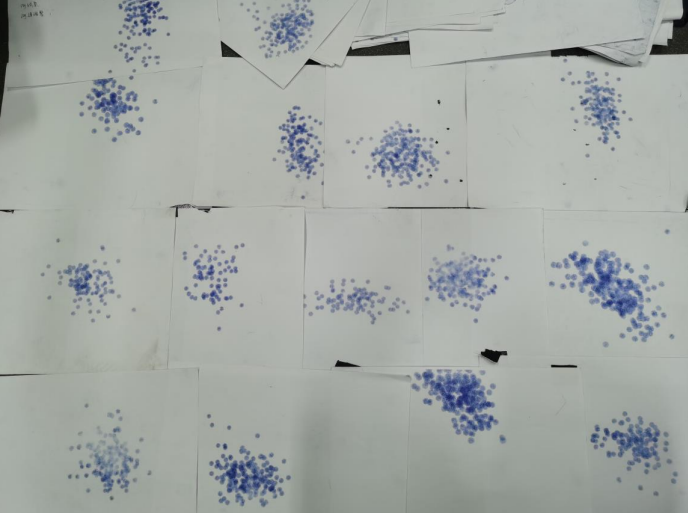
\includegraphics[width=0.5\columnwidth]{figure/研发迭代过程/重复度结果展示图-1.png}
    }
    \subfigure[重复度结果展示图2]{
        \centering
        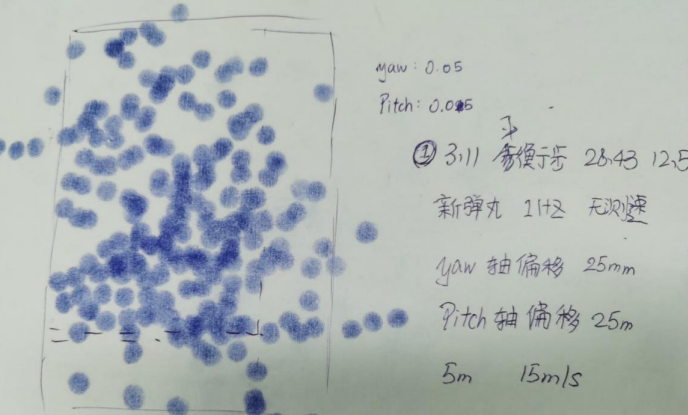
\includegraphics[width=0.5\columnwidth]{figure/研发迭代过程/重复度结果展示图-2.png}
    }
    \caption{重复度测试结果展示}
    \label{fig:重复度结果展示图}
\end{figure} 